\chapter{Realizace gatewaye}

\section{Výběr přenosové technologie}
Pro tento systém je použita RF technologie LoRa se standardizovaným síťovým protokolem LoRaWAN, ale s požitím pouze jednoho kanálu.
Jedenokanálové řešení bylo zvoleno z toho důvodu, že plnohodnotný LoRa transceiver, který prijímá na všech osmi kanálech je příliš drahý (přibližně desetinásobná cena) a složitý k implementaci, zatímco v tomto projektu je kladen důraz na cenu a jednoduchost řešení.

Vybraná technologie používá topologii typu hvězda, tedy koncová zařízení komunikují přímo s gatewayí, zbýtek času mohou být ve stavu nízké spotřeby, což má za důsledek delší životnost baterie.
Koncová zařízení od různých výrobců jsou plně kompatibilní s cizí gatewayí, tudíž není problém je implementovat do tohoto systému. Je pouze třeba je překonfigurovat pro vysílání na jednom použitém kanále.

todo

\subsection{Zabezpečení protokolu LoRaWAN}
Protokol LoRaWAN používá AES-128 na 2 způsoby, pro síťové a aplikační zabezpečení. Jsou zde tedy 2 šifrovací klíče, NwkSKey a AppSKey.

\subsubsection{Síťové zabezpečení}
Síťové zabezpečení je zde aby bylo hackerům zabráněno odesílání duplikovaných packetů nebo vytváření a vysílání packetů s nasimulovanými daty.
Poslední 4 byty packetu obsahují MIC (Message Integrity Code), který je získán zašifrováním dat síťovým klíčem NwkSKey obsahujících mimo jiné celý payload packetu (včetně packet counter). Toto umožňuje odhalit jakoukoliv manipulaci s daty v packetu. LoRaWAN packet také obsahuje counter počítající od nuly od doby kdy bylo LoRaWAN zařízení spuštěno. Toto umožňuje odhalit duplikování packetů.


\subsubsection{Aplikační zabezpečení}
Aplikační klíč AppSKey (Application Session Key) je použit pro zašifrování dat aplikační zprávy (App message) \cite{lwSpec} \cite{lwSecur}.


%%%%%%%%%%%%%%%%%%%%%%%%%%%%%%%%%%%%%%%%%%%%%%%%%%%%%%%%%%%%%%%%%%%%%%%%%%
\section{Výběr komponent}
\subsection{Microcontroller}
Pro toto zařízení je zvolen mikrocontroller STM32L073RZ se zaměřením na nízkou spotřebu, jelikož je levný, má dostačující vlastnosti a je dostupný ve formě vývojového kitu NUCLEO-L073RZ který byl použit pro  vývoj zařízení. Mezi hlavní vlastnosti patří \cite{nucleoST}:
\begin{itemize}    
    \item {Architektura ARM Cortex-M0+ 32-bit RISC}
    \item{Interní Flash paměť 192 KB}
    \item{Interní SRAM paměť 20 KB}
    \item{Interní EEPROM paměť 6 KB}
    \item {Až 32 MHz CPU}
    \item {2X SPI, 3x I2C, 4x USART, LIN, ADC}
\end{itemize}

Pořizovací cena kitu přímo na stránce výrobce www.st.com je \$13 \cite{nucleoST} \cite{nucleoMbed}.
\begin{figure}[!h]
    \centering
    \includegraphics[width=0.4\textwidth]{Nucleo64}
    \caption{Vývojový kit NUCLEO-L073RZ \cite{nucleoST}}
    \label{fig:02}
\end{figure}

\subsection{LoRa transceiver}
Lora transceiver čip doposud vyrábí pouze Semtech, pro použití v Evropském pásmu je určen typ SX1276.
V tomto návrhu je použita deska RFM95w od firmy HopeRF s integrovaným čipem SX1276 \cite{RFM95w}.
Pro vývoj zařízení byl využit tento transciever v tzv. Dragino LoRa Shield \cite{draginoWiki}, který má stejně jako použitý vývojový kit, pinout kompatibilní s Arduino UNO. Pořizovací cena samotného transceiveru RFM95w je okolo \$7, cena Dragino Shieldu se pohybuje okolo \$22 na ebay.

\begin{figure}[!h]
    \centering
    \includegraphics[width=0.2\textwidth]{RFM95w}
    \caption{LoRa transceiver RFM95w \cite{RFM95w}}
    \label{fig:02}
\end{figure}

\subsection{RS485 transceiver}
SparkFun Transceiver Breakout - RS485 převádí rozhranní UART na RS485, pří vstupním napětí 3.3 V. A je dostupný za cenu okolo \$10 \cite{rs485tr}.

\begin{figure}[!h]
    \centering
    \includegraphics[width=0.4\textwidth]{rs485transceiver}
    \caption{RS485 transceiver \cite{rs485tr}}
    \label{fig:rs485transceiver}
\end{figure}



\newpage
%%%%%%%%%%%%%%%%%%%%%%%%%%%%%%%%%%%%%%%%%%%%%%%%%%%%%%%%%%%%%%%%%%%%%%%%%
\section{Implementace LoRaWAN sítě}
Jednokanálové použití technologie LoRa umožňuje použít transceiver navržený pro koncová zařízení, 
kterým jsou packety kontinuálně odposlouchávány na jednom nastaveném kanále a SF. Tyto dva parametry  jsou nakonfigurovány na všech koncových zařízeních v síti.

Použitý protokol IMA\_RS485, původně navržen pro přístupové systémy, umožňuje posílat data pouze pomocí příkazu "průchod", který má kapacitu pro data z koncového zařízení pouze 6 B. Systém je proto navržen neobvyklým způsobem. Přijme-li gateway LoRaWAN packet, nejprve zkontroluje zda zná adresu zařízení, pokud ano, přečte z paměti i typ zařízení, packet dešifruje a dekóduje payload, čímž získá konečné hodnoty senzorů, které pak dále pošle přes RS485 rozhraní na server.
LoRaWAN device address a typ každého zařízení v síti je uložena v EEPROM (non-volatile) paměti gatewaye a jsou nastavována na K4 serveru.
Všechna zařízení mají nastavené stejné šifrovací klíče a gateway je má uložené v EEPROM.

Pro tento projekt byla vyvinuta knihovna pro dekódování payloadu na základě dokumentů \cite{lwSpec} \cite{lwSecur}.


%%%%%%%%%%%%%%%%%%%%%%%%%%%%%%%%%%%%%%%%%%%%%%%%%%%%%%%%%%%%%%%%%%%%%%%%%%
\section{Implementace komunkičního protokolu v síti IMA\_RS485}
V tomto projektu je komunikace protokolu IMA\_RS485 naprogramována v souborech rs485\_protocol.h a rs485\_protocol.c. Jedná se o kolizní protokol v síti, kde je připojen jeden master, a jeden nebo více slaveů řízených masterem.

\begin{table}[!h]
    \centering
    \begin{tabular}{ |c|c| }
     \hline

     Baud rate              & 9600           \\ \hline
     Data bits              & 8                 \\ \hline
     Parity                 & none              \\ \hline
     Stop bits              & 1                 \\ \hline

    \end{tabular}
    \caption{Fyzické vlastnosti IMA\_RS485 sítě}
    \label{table:3}
\end{table}

\newpage
\subsection{Syntaxe příkazů}
Komunikace v síti probíha formou příkazů, které mají specifikovanou syntaxi v tabulce \ref{table:syntaxePrikazu}.

\begin{table}[!h]
    \centering
\begin{tabular}{ |c|| p{1.5cm} | p{1.5cm} | p{1cm} | p{1cm} | p{1cm} | p{1cm} | }
 \hline
 popis      & adresa příjemce & adresa odesílatele & typ příkazu & délka dat & data & crc\\ \hline
 počet bytů & 1               & 1   & 1     & 2     & délka dat     & 1 \\ 
 \hline
\end{tabular}
    \caption{Syntaxe příkazu pro komunikaci v síti IMA\_RS485}
    \label{table:syntaxePrikazu}
\end{table}

Typy příkazu jsou zadefinované konstanty s předponou CKP\_CMD\_ v souboru ./Inc/rs485\_protocol.h.
Příkazy odeslané masterem obsahují navíc synchronizační byte na začátku 0xAA.
CRC je pro kontrolu XOR přes všechny předchozí byty v celém příkazu kromě synchronizačního bytu.

\subsection{Adresace zařízení v síti}
Každé zařízení na této sběrnici má svoji adresu, která mu je nastavena externě. Master má adresu  0xFF, adresa pro všechny (broadcast) je 0x00 a zařízení v této sítí můžou mít adresu libovolnou (krom těchto dvou) nesmí zde však být připojena 2 zařízení s nastavenou stejnou adresou.

\subsection{Statusy}
Slave má dva možné statusy, offline a online, což značí, zda je zařízení v aktivním režumu, tudíž má povolení odesílat příkaz průchod (V případě této gatewaye příkaz průchod obsahuje data ze koncového zařízení).  
Slave odesílá příkoz obsahující onformaci o jeho statusu periodicky s typem příkazu 0x10 a jedním bytem dat označujícím status. Master na tento příkaz odpoví pouze pokud mění status slaveu. Pokud je slave online a master přestane komunikovat, zařízení slave se samo přepne na status offline.

\subsubsection{Offline}
Je-li zařízení zapnuto, je ve stavu offline. Nemá povoleno odesílat příkaz průchod obsahující data z koncových zařízení, pouze odpovídá na příkazy masteru. Odesílání příkazu signalizující tento stav je s periodou 10 s a obsahuje byte 0xEE.

\subsubsection{Online}
Odesílání příkazu signalizující tento stav je s periodou 45 s a obsahuje byte 0x00.
V tomto stavu je povoleno odesílání příkazu průchod.


\subsection{Přidávání LoRaWAN zařízení do systému}
Pokud master přijme od slavea příkaz oznamující že je ve stavu offline, nejprve slaveu pošle seznam LoRaWAN adres všech známých koncových zařízení a následně slavea přepne do stavu online.
Přijímání seznamu adres je realizov8no sekvencí příkazů typu 0x8F. 

Níže v tabulce \ref{table:2} je příklad sekvence příkazů odesílaných mezi masterem a slavem během předávání seznamu LoRaWAN device address koncových zařízení, kde slave má adresu 0x10 a master standartně 0xFF. Jak již bylo řečeno, příkazy od serveru lze jednoduše odlišit tím, že vždy začínají bytem 0xAA.


\begin{table}[!h]
    \begin{tabular}{ |l|p{10cm}| }
    \hline
    příkaz      &  data    \\ \hline \hline
    start      &  AA 10 FF 8F 02 00 00 00 62    \\ \hline
    ACK        &  FF 10 06 02 00 8F 00 64    \\ \hline
    data     &  AA 10 FF 8F 21 00 01 B1 C4 12 00 00 00 00 00 B2 C4 12 00 00 00 00 00 B3 C4 12 00 00 00 00 00 B4 C4 12 00 00 00 00 00 44 \\ \hline
    ACK      &  FF 10 06 02 00 8F 01 65   \\ \hline
    data     &  AA 10 FF 8F 19 00 02 B5 C4 12 00 00 00 00 00 B6 C4 12 00 00 00 00 00 F6 1F 01 26 00 00 00 00 B6 \\ \hline
    ACK      &   FF 10 06 02 00 8F 02 66   \\ \hline
    konec      &   AA 10 FF 8F 04 00 03 FF 2A 57 E5   \\ \hline
    ACK      &   FF 10 06 02 00 8F 03 67  \\ \hline
    \end{tabular}
    \caption{Příklad sekvence příkazů odesílaných mezi masterem a slavem během předávání seznamu LoRaWAN device address koncových zařízení}
    \label{table:2}
\end{table}

LoraWAN protokol používá 4-bytové adresy koncových zařízení.
Adresy předávány touto sekvencí jsou dlouhé 8-bytové. První 4 byty je tedy LoRaWAN device address, páty byte je typ zařízení a zbylé 3 byty jsou nevyužity, jejich použití je možné v případě změn či rozšiřování vlastností systému. 

První Byte dat je counter packetu začínající od nuly, který označuje číslo odeslaného packetu v sekvenci. Na každý tento packet v sekvenci slave odpovídá ACK příkaz, který se liší od obyčejného ACK příkazu tím, že v datech packetu navíc obsahuje counter packety v sekvenci.
První příkaz této sekvence má délku dat 2 byty, které mají hodnotu 0x00 přičemž první je counter.
Další příkazy hned za counter bytem obsahují několik osmibytových adres, jejichž počet je různý.
Příkaz ukončující tuto sekvenci příkazů má délku 4 byty, což je tedy counter, 0xFF a 2 byty CRC přes všechny odeslané adresy (nepodstatné, tudíž ho nepoužívám).

\subsection{Odesílání dat ze senzoru}
todo
Jak již bylo zmíněno, protokol byl navrhnut pro přístupové systémy a nedošlo k žádné úpravě pro tuto odlišnou aplikaci. Data ze senzorů se tedy posílají s použitím stávajícího příkazu "průchod".
Typ tohoto příkazu je 0x10. První byte dat označuje typ průchodu, byl zvolen konstantní byte 0xD0.
Dále následuje LoRaWAN adresa modulu od kterého byl přijat packet. Dále následují 4 byty dat ze senzoru. Dále 2 byty oznamující čas průchodu, což v tomto projektu není použito a tyto dva byty mají tedy hodnotu 0xFF. A nakonec jsou další 2 byty obsahující data ze senzoru.
Celý tento příkaz průchod tedy obsahuje pouze 6 bytů pro data ze senzoru.

Server na tento příkaz odpovídá ACK a má čas na odpověď standardně 3 sekundy, ale tento parametr je nastavitelný. Pokud v tomto timeoutu neodpoví, zařízení  příkaz zopakuje a změní typ příkazu na 0x20. Pokud server ani na třetí opakování neodpoví ACK, zařízení se přepne do stavu offline a vymaže frontu příkazů k odeslání.

\subsection{Potvrzení}
Zařízení odpovídá na každý platný příkaz od serveru ACK. Typ příkazu ACK je 0x06 a v datech je jeden byte, což je typ příkazu na který právě odpovídá potvrzením.
\\ \\
Server odpovídá ACK se stejným typem příkazu 0x06, ale s žádnými daty v příkazu. Délka dat je tedy 0.

\subsection{Dotaz na příznaky}
Server se může zeptat s jak dlouhýmí adresami zařízení pracuji. Je to typ příkazu 0x49 a délka dat je 0. Zařízení na to odpoví ACK, ale navíc je v datech příkazu byte 0x04 a server pak počítá s tím, že pracuji se 64-bit adresami (ve skutečnosti ale používám 32-bitové a zbylé 4 byty jsou pro data).


%%%%%%%%%%%%%%%%%%%%%%%%%%%%%%%%%%%%%%%%%%%%%%%%%%%%%%
\section{Paměť}
Konfigurace systému, DevAddr a typ všech zařízení v síti jsou uložena v non-volatile paměti procesoru EEPROM, která je o velikosti 6144 B. 
Paměť je tedy rozdělená tak, že od adresy 0 až po 6080 je prostor pro ukládání LoRaWAN zařízení a od 6080 až po 6144 je prostor pro ukládání konfigurace systému.

Každé LoRaWan zařízení v síti má v paměti uložené device address (4 byty), typ zařízení (1 byte) a další 3 byty jsou rezervovány. 
Jedno zařízení zabírá tedy 8 B, takže jich pro jednu síť může být až 760.


%%%%%%%%%%%%%%%%%%%%%%%%%%%%%%%%%%%%%%%%%%%%%%%%%%%%%%
\section{Komunikace přes USB}
Komunikace přes USB s PC má za účel konfiguraci systému a Log aplikace. Lze k tomu použít libovolný terminál s nastavením viz tabulka \ref{table:2}.

\begin{table}[!h]
    \centering
    \begin{tabular}{ |c|c| }
     \hline

     Baud rate              & 115200           \\ \hline
     Data bits              & 8                 \\ \hline
     Parity                 & none              \\ \hline
     Stop bits              & 1                 \\ \hline
     Flow control           & none               \\ \hline

    \end{tabular}
    \caption{Nastavení USB terminálu}
    \label{table:3}
\end{table}

Při komunikaci jsou data oddělována bytem 0x0D, ale je akceptována i sekvence 0x0D 0x0A. 

\subsection{Log aplikace}
Gateway odesílá informace přes USB o tom, co právě provádí. Níže je příklad výpisu dat pro případ, že gateway přijme packet. Nejprve jsou vypsána data týkající se LoRaWAN protokolu, DevAddr bylo rozpoznáno, payload byl dešifrován a na základě typu senzoru byl dekódován payload a vyčteny hodnoty senzorů LoRaWAN zařízení. Poslední řádek obsahuje data odeslané přes RS485 na server.


\begin{lstlisting}
______________________________________________________
Rx -> LoRaWAN, pktCntr: 406
RSSI: -29, SNR: 9, length: 22
Packet rawData:  40 F6 1F 01 26 C0 A1 30 08 D4 5D 93 F0 F0 F6 60 C0 04 BC BE 4B 24
devAddr:  F6 1F 01 26
MHDR: 40
FCtrl: c0
FCnt: 12449
FPort: 08
MIC:  BC BE 4B 24
adaptive data rate:  1
ack: 0
direction: UP
message (encrypted):  D4 5D 93 F0 F0 F6 60 C0 04
message (decrypted):  01 44 6C 83 05 00 FF FF 71

Sensor type: RHF1S001
temperature: 27.46 C, humidity: 58 %
period: 10 s, RSSI: -29 dBm, SNR: 9 dB, battery voltage: 2.6 V
Tx -> RS-485: " FF 10 10 0D 00 D0 F6 1F 01 26 BA 0A 3A E3 FF FF 09 1A 96"
\end{lstlisting}

\subsection{Konfigurace systému}
Pro vstup do configuration setup menu musí být odeslán příkaz "config". Z menu je možné vystoupit kdykoliv příkazem "quit" (bez uložení). 
Při vstupu do stavu konfigurace systému je pozastavena činnost gatewaye (přijímání LoRaWAN packetů, komunikace se serverem,...).
V terminálu je nejprve vypsána kompletní aktuální konfigurace systému a následně menu konfigurace. Uživatel pak vybírá zadáním čísla.
Níže je zobrazen příklad výpisu po vstupu do konfigurace.
\\

\begin{lstlisting}

_________________Entering configuration setup________________


System configuration:

*** LoRa channel: 
channel: 0 (868.1 Mhz)
SF7

*** RS485 channel: 
my address: 10
server address: FF
timeout: 3 s

*** LoRaWAN keys: 
NwSKey:  FD 90 0D 8C 70 9F 19 24 18 EC FD D4 28 0C AC 47
AppSKey:  68 9F D0 AC 7A 0F 95 58 B1 19 A0 16 17 F4 16 33


Config menu:
1 -> Config LoRa channel
2 -> Config RS485 channel
3 -> Config LoRaWAN protocol
4 -> Print all LoRaWAN devices
5 -> Erase all LoRaWAN devices
6 -> Restore to default configuration
7 -> Exit without save
8 -> Save and exit
\end{lstlisting}



Jsou zde tedy 3 stavy konfigurace, přičemž je možné vždy jednotlivá nastavení přeskakovat odesláním "prázdného příkazu" 0x0D (v terminálu obvykle stačí stisknout Enter). Systém při konfiguraci vždy vypíše jaká data mají být zadána v jakém tvaru a zároveň současnou hodnotu měněného parametru. Zadaná data uživatelem jsou vždy zkontrolována zda splňují požadovaný tvar. Pokud ne, uživatel je o tom informován a vyzván k dalšímu pokusu.
Po provedení konfigurace následuje vždy návrat do menu. Pro uložení nové konfigurace je potřeba v menu vybrat "Save and exit", systém pak následně vypíše které parametry byly změněny.

\subsubsection{Config LoRa channel}
Konfigurace LoRa RF kanálu zahrnuje nastavení SF a frekvenční pásmo. Níže je příklad konfigurace.

\begin{lstlisting}
LoRa channel configuration:
Enter SF number (7-12)
(current: 7)
8
SF8 set.

Enter LoRa channel number (0-7)
ch0 is 868.1 Mhz
ch1 is 868.3 Mhz
ch2 is 868.5 Mhz
ch3 is 867.1 Mhz
ch4 is 867.3 Mhz
ch5 is 867.5 Mhz
ch6 is 867.7 Mhz
ch7 is 869.0 Mhz
(current: 0)
1
channel 1 set.
\end{lstlisting}


\subsubsection{Config RS485 channel}
Konfigurace RS485 kanálu pro komunikaci se serverem zahrnuje nastavení adresy tohoto zařízení, adresa serveru a timeout, což je doba čekání na zprávu ACK od serveru po odeslání příkazu obsahujícího data ze senzorů. Níže je příklad konfigurace.

\begin{lstlisting}
RS485 channel configuration:
Enter address of this device, FF and 00 are reserved.
(current: 10)
11
Address of this device is set to: 11

Enter server address: 
(current: FF)
FE
Server address is set to: FE

Enter timeout (seconds)
(current: 3)
5
timeout set to: 5 s
\end{lstlisting}


\subsubsection{Config LoRaWAN protocol}
Konfigurace LoRaWAN zahrnuje nastavení šifrovacích klíčů pro LoRaWAN protokol. Níže je příklad konfigurace.

\begin{lstlisting}
LoRaWAN protocol configuration:
Enter NwSKey (16 bytes in HEX)
(current:  FD 90 0D 8C 70 9F 19 24 18 EC FD D4 28 0C AC 47)
11111111222222223333333344444444
NwSKey set to: 11 11 11 11 22 22 22 22 33 33 33 33 44 44 44 44

Enter AppSKey (16 bytes in HEX)
(current:  68 9F D0 AC 7A 0F 95 58 B1 19 A0 16 17 F4 16 33)
11111111222222223333333344444444
AppSKey set to: 11 11 11 11 22 22 22 22 33 33 33 33 44 44 44 44
\end{lstlisting}




\subsubsection{Print all LoRaWAN devices}
Vypíše všechna LoRaWAN zařízení uložená v paměti. Níže je příklad.


\begin{lstlisting}
number.......................0:
Device Address:  B1 C4 12 00
Device Type: RH1S001
number.......................1:
Device Address:  B2 C4 12 00
Device Type: RH1S001
number.......................2:
Device Address:  B3 C4 12 00
Device Type: RH1S001
number.......................3:
Device Address:  B4 C4 12 00
Device Type: IMA_tempPress
number.......................4:
Device Address:  B5 C4 12 00
Device Type: IMA_tempPress
\end{lstlisting}



\subsubsection{Restore to default configuration}
Po zvolení této možnosti je načtena defaultní konfigurace systému, která obsahuje hodnoty viz tabulka \ref{table:5}.

\begin{table}[!h]
    \centering
    \begin{tabular}{ |l|l| }
     \hline

     popis              & hodnota         \\ \hline \hline
     RS485 myAddr       & 0x10            \\ \hline
     RS485 serverAddr   & 0xFF            \\ \hline
     RS485 timeout      & 3               \\ \hline
     LoRa SF            & SF7             \\ \hline
     LoRa channel       & 0 (868.1 Mhz)   \\ \hline
     NwSKey             & FD 90 0D 8C 70 9F 19 24 18 EC FD D4 28 0C AC 47  \\ \hline
     AppSKey            & 68 9F D0 AC 7A 0F 95 58 B1 19 A0 16 17 F4 16 33  \\ \hline

    \end{tabular}
    \caption{Defaultní konfigurace systému}
    \label{table:5}
\end{table}


\newpage
%%%%%%%%%%%%%%%%%%%%%%%%%%%%%%%%%%%%%%%%%%%%%%%%%%%%%%
\section{Koncová zařízení}
Jelikož používaný protokol ke komunikaci se serverem je datově omezen na 6B na jeden paket, payload senzoru je dekódován v gatewayi a v packetu odeslaném na server jsou pouze nejdůležitější data, která se vejdou do této velikosti.
Na základě typu koncového zařízení jsou data v packetu zakódovány, tudíž typ koncového zařízení musí být v gatewayi implementován.
Typ kobncového zařízení je definován jedním bytem a je uložen v gatewayi i na serveru společně s DevAddr u každého koncového zařízení.

Momentálně jsou podporovány dva typy koncových zařízení, dle potřeby neni problém rozšířit FW gatewaye o další typy koncových zařízení.

\begin{table}[!h]
    \centering
    \begin{tabular}{ |l|l| }
     \hline

     Typ zařízení       & Hodnota         \\ \hline \hline
     RHF1S001           & 0x00            \\ \hline
     IMA\_tempPress     & 0x01            \\ \hline
     
    \end{tabular}
    \caption{Typy koncových zařízení}
    \label{table:TypyKoncZarizeni}
\end{table}

\subsection{Zpracování dat jednotlivých typů koncových zařízení}
Níže je popsáno pro jednotlivá koncová zařízení jak jsou data uložena ve struktuře, jak jsou data z této struktury zpracována a zobrazena a nakonec jak vybraná data jsou zapsána do výsledného bufferu o délce 6B, který je odeslán na K4 server

\subsubsection{RHF1S001}
Senzor od firmy RisingHF měří teplotu a vlhkost.

\begin{lstlisting}[style=CStyle]
    /* RHF1S001 data structure */   
    typedef struct {
        int16_t temperature;
        uint8_t humidity;
        uint16_t period;
        int8_t rssi;
        int8_t snr;
        uint8_t battery;
    } RHF1S001_data_t;

    /* Print the data from the structure */
	printf("temperature: %d.%d C, ", RHF1S001_data.temperature / 100, RHF1S001_data.temperature % 100);
	printf("humidity: %d %%\n", RHF1S001_data.humidity);
	printf("period: %d s, ", (int)RHF1S001_data.period);
	printf("RSSI: %d dBm, ", RHF1S001_data.rssi);
	printf("SNR: %d dB, ", RHF1S001_data.snr);
	printf("battery voltage: %d.%d V\r\n", RHF1S001_data.battery/10, RHF1S001_data.battery % 10);

    /* Put the data into 6B long buffer, that is transmitted to the K4 server */
	buffer[0] = RHF1S001_data.temperature & 0xFF;
	buffer[1] = RHF1S001_data.temperature >> 8;
	buffer[2] = RHF1S001_data.humidity;
	buffer[3] = RHF1S001_data.rssi;
	buffer[4] = RHF1S001_data.snr;
	buffer[5] = RHF1S001_data.battery;
\end{lstlisting}


\subsubsection{IMA\_tempPress}
Senzor vytvořený ve firmě IMA, měřící teplotu a tlak.

\begin{lstlisting}[style=CStyle]
    /* IMA_tempPress data structure */   
    typedef struct {
        int16_t temperature;
        uint16_t pressure;
        int8_t rssi;
        int8_t snr;
    } IMA_tempPress_data_t;
    
    /* print the data from the structure */
	printf("temperature: %d.%d C, ", IMA_tempPress_data.temperature / 100, IMA_tempPress_data.temperature % 100);
	printf("pressure: %d.%d Pa\r\n", IMA_tempPress_data.pressure/10, IMA_tempPress_data.pressure % 10);
	printf("RSSI: %d dBm, SNR: %d dB\r\n", IMA_tempPress_data.rssi, IMA_tempPress_data.snr);

    /* Put the data into 6B long buffer, that is transmitted to the K4 server */
	buffer[0] = IMA_tempPress_data.temperature & 0xFF;
	buffer[1] = IMA_tempPress_data.temperature >> 8;
	buffer[2] = IMA_tempPress_data.pressure & 0xFF;
	buffer[3] = IMA_tempPress_data.pressure >> 8;
	buffer[4] = IMA_tempPress_data.rssi;
	buffer[5] = IMA_tempPress_data.snr;
\end{lstlisting}


\subsection{Přidávání koncových zařízení ze serveru K4}
Koncocová zařízení sítě se nastavují ze serveru K4 v podobě seznamu offline karet s délkou UID 8B.
LoRaWAN device address je dlouhá 4B, jeden byte je navíc použit pro typ koncového zařízení, zbylé 3 byty jsou nuly.
Jelikož typ zařízení je uložen v gatewayi i na serveru. Při odesílání zprávy průchod se tedy už typ zařízení neposílá z důvodu datového omezení v této zprávě (6B).
Na serveru K4 se UID nastavuje jako dekadické číslo.
Níže je příklad vytvoření výsledného čísla obsahující DevAddr a typ zařízení, které se zadává do K4 serveru.

\subsubsection{Příklad}
Pro případ, kde typ zařízení je 01 a DevAddr AABBCCDD (little endian) výsledné číslo v hexadecimální podobě je 01DDCCBBAA. Následně se překládá do decimalni podoby, výsledné číslo k zadání do K4 serveru je tedy 8016149418.


\newpage
%%%%%%%%%%%%%%%%%%%%%%%%%%%%%%%%%%%%%%%%%%%%%%%%%%%%%%
\section{Zapojení}
LoRa shield \cite{draginoWiki} je nasazen přímo na vývojový kit. 
Nukleo kit neobsahuje ISCP konektor, který je součástí pinoutu Arduina a LoRa shield má SPI piny MISO a MOSI přivedeny právě na tento konektor. Musí být tedy propojeny externě viz obrázek \ref{fig:03}.
Jumpery na shieldu musí také být stejně jako v obrázku.

% \begin{figure}[!h]
%     \centering
%     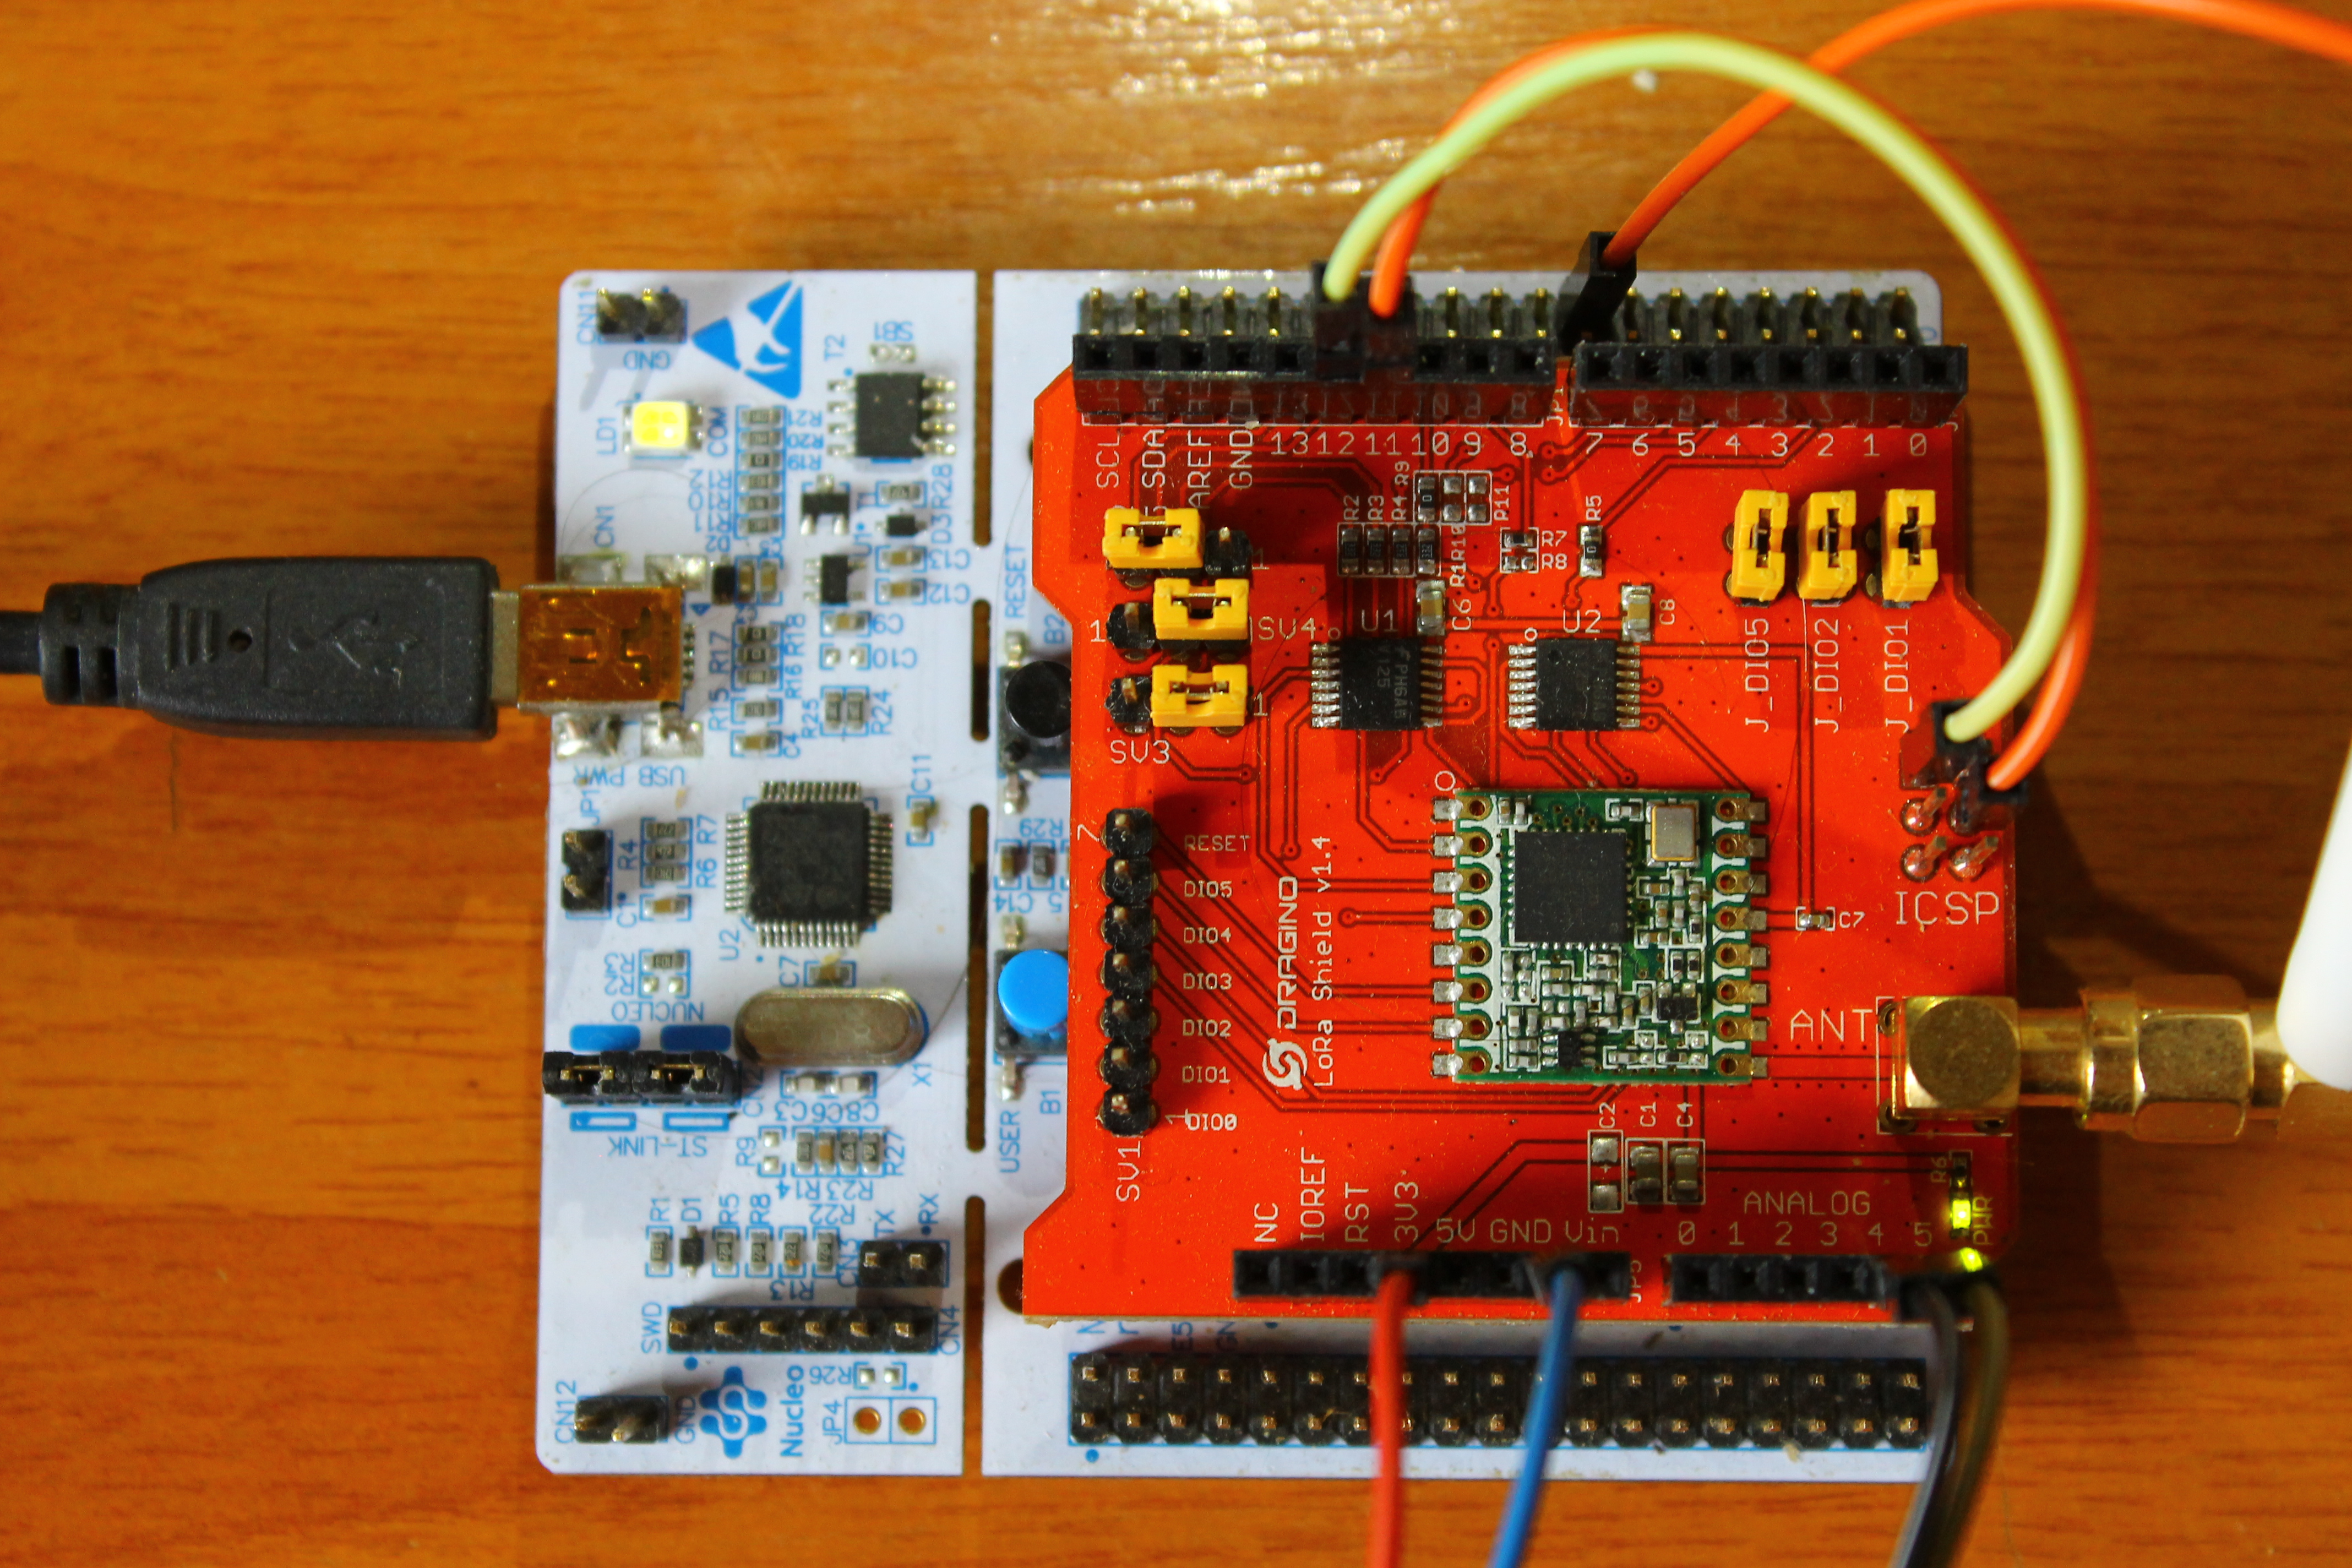
\includegraphics[width=1\textwidth]{foto01.jpg}
%     \caption{foto zapojení}
%     \label{fig:03}
% \end{figure}


Pro komunikaci s LoRa transceiverem je tedy použito SPI1, pro komunikaci přes USB je použito USART2 a pro komunikaci přes RS485 je použito UART1.


\begin{table}[h]
    \centering
    \begin{tabular}{ |c|c|c| }
     \hline

     Periférie          & Název pinu & Pin procesoru           \\ \hline \hline
     
                        & RX  &   PC1            \\
    RS485 transceiver   & TX  &   PC0       \\
                        & RTS  &  PB1      \\     \hline

                        & CS    &  PB6             \\
                        & CLK   &  PA5        \\
   LoRa transceiver     & MISO  &  PA6     \\
                        & MOSI  &  PA7        \\
                        & RST   & PC7          \\
                        & DIO0  & PA10         \\
                        \hline

    \end{tabular}
    \caption{Pinout připojení externích periférií k procesoru}
    \label{table:3}
\end{table}


\section{Instalace}
K nahrání zkompilovaného programu do procesoru z PC není potřeba instalovat žádný SW. 
Kit je potřeba připojit k PC přes USB. V PC se to zobrazí jako flash disk. Zkompilovaný program s koncovkou .binary stačí překopírovat na toto zařízení. Po dobu kopírování souboru bliká na kitu LED1 červená/zelená. Jakmile kopírování skončí, program se spustí. Kit je také možné restartovat černým tlačítkem reset.

 Pro uvedení Gatewaye do provozu je nutné se připojit k zařízení přes USB a nastavit všechny parametry viz sekce v tomto dokumentu: "Konfigurace systému".

\newpage
%%%%%%%%%%%%%%%%%%%%%%%%%%%%%%%%%%%%%%%%%%%%%%%%
\section{Zdrojové soubory projektu}
Projekt byl naprogramován v AtolicTrueSTUDIO, což je IDE založené na Eclipse. 
K programování procesoru byly použity standartní HAL knihovny od firmy ST Microelectronics.
Pro šifrování LoRaWAN packetu byla použita knihovna AES-128, dostupná na githubu \cite{AESlib} a knihovna OpenPANA také dostupná z githubu \cite{CMAClib}.
Níže je seznam zdrojových souborů.

\begin{figure}[!h]
    \dirtree{%
        .1 Drivers \DTcomment{STM32 Drivers}.
        .1 Inc\DTcomment{Headers}.
            .2 aes.h\DTcomment{AES-128 library for LoRaWAN packet encryption}.
            .2 cmac.h\DTcomment{library for CMAC calculation in LoRaWAN protocol}.
            .2 LinkedList\_ByteArray.h \DTcomment{Byte array linked list library for stacks}.
            .2 LoRaWAN\_packet.h\DTcomment{LoRaWAN library for packet data decoding}.
            .2 stm32l0xx\_hal\_conf.h\DTcomment{STM32 HAL library}.
            .2 ByteArray.h\DTcomment{Library for Byte array operations}.
            .2 LoRa.h\DTcomment{Library for interfacing LoRa transceiver}.
            .2 main.h\DTcomment{Main file}.
            .2 stm32l0xx\_it.h\DTcomment{STM32 HAL library}.
            .2 eeprom.h\DTcomment{Library for eeprom operations}.
            .2 LoRa\_sensors.h\DTcomment{Library for decoding data from payload}.
            .2 rs485\_protocol.h\DTcomment{Library for RS485 IMA protocol}.
            .2 usb.h \DTcomment{Library for USB communication and system configuration}.
        .1 Src\DTcomment{Sources}.
            .2 aes.c \DTcomment{source file to the aes.h}.
            .2 aes.c \DTcomment{source file to the cmac.h}.
            .2 LinkedList\_ByteArray.c \DTcomment{source file to the LinkedList\_ByteArray.h}.
            .2 LoRaWAN\_packet.c  \DTcomment{source file to the LoRaWAN\_packet.h}.
            .2 stm32l0xx\_hal\_msp.c \DTcomment{HAL source file}.
            .2 ByteArray.c  \DTcomment{source file to the ByteArray.h}.
            .2 LoRa.c \DTcomment{source file to the LoRa.h}.
            .2 main.c \DTcomment{main source file}.
            .2 stm32l0xx\_it.c \DTcomment{HAL source file}.
            .2 eeprom.c \DTcomment{source file to the eeprom.h}.
            .2 LoRa\_sensors.c \DTcomment{source file to the LoRa\_sensors.h}.
            .2 rs485\_protocol.c  \DTcomment{source file to the rs485\_protocol.h}.
            .2 system\_stm32l0xx.c \DTcomment{HAL source file}.
            .2 usb.h \DTcomment{source file to the usb.h}.
    }
\end{figure}

